% figures/campaign-hierarchy.tex
% Standalone TikZ: Google vs Meta campaign hierarchy (ch.09 paid acquisition).
% Compiled to figures/campaign-hierarchy.pdf via tools/build-figures.sh.
\documentclass[tikz,border=4pt]{standalone}
\usepackage{tikz}
\usetikzlibrary{arrows.meta,positioning}

% Palette matching preamble.sty tcolorbox colours
\definecolor{gblue}{HTML}{1A5276}   % Google column (blue!55!black)
\definecolor{mteal}{HTML}{0E6655}   % Meta column (teal!60!black)
\definecolor{lvl}{HTML}{4D4D4D}

\begin{document}
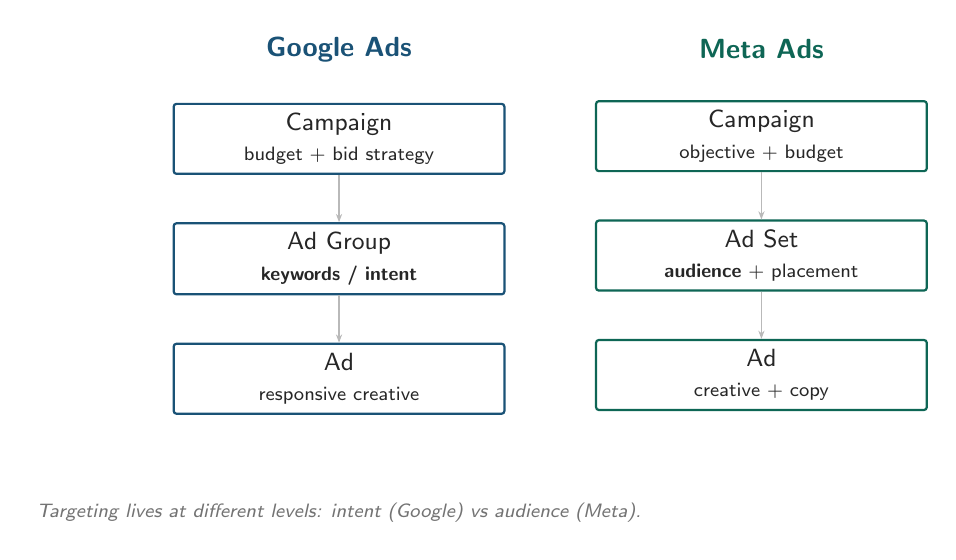
\begin{tikzpicture}[
  node distance=6mm,
  box/.style={draw=#1, line width=0.8pt, rounded corners=1pt, text=black!85,
              font=\sffamily\small, minimum width=42mm, minimum height=8mm, align=center},
  lbl/.style={font=\sffamily\bfseries, text=#1},
  ar/.style={-{Stealth[length=3pt]}, gray!55},
]
% Column headers
\node[lbl=gblue] (gh) {Google Ads};
\node[box=gblue, below=4mm of gh] (g1) {Campaign\\{\scriptsize budget + bid strategy}};
\node[box=gblue, below=of g1] (g2) {Ad Group\\{\scriptsize \textbf{keywords / intent}}};
\node[box=gblue, below=of g2] (g3) {Ad\\{\scriptsize responsive creative}};
\draw[ar] (g1) -- (g2);
\draw[ar] (g2) -- (g3);

% Meta column
\node[lbl=mteal, right=34mm of gh] (mh) {Meta Ads};
\node[box=mteal, below=4mm of mh] (m1) {Campaign\\{\scriptsize objective + budget}};
\node[box=mteal, below=of m1] (m2) {Ad Set\\{\scriptsize \textbf{audience} + placement}};
\node[box=mteal, below=of m2] (m3) {Ad\\{\scriptsize creative + copy}};
\draw[ar] (m1) -- (m2);
\draw[ar] (m2) -- (m3);

% Targeting-level callout
\node[font=\sffamily\scriptsize\itshape, text=black!55, below=10mm of g3] (cap)
  {Targeting lives at different levels: intent (Google) vs audience (Meta).};
\end{tikzpicture}
\end{document}
